\documentclass[a4paper]{article}
\usepackage[utf8]{inputenc}
\usepackage[IL2]{fontenc}
\usepackage[czech]{babel}
\usepackage{amsmath}
\usepackage{fullpage}
\usepackage[pdftex]{graphicx}

\usepackage[pdftex,unicode,hidelinks]{hyperref}

\title{Lambert-CZ -- nové zobrazení pro Česko}
\date{\today}
\author{Jan Šimbera}

\newcommand{\file}[1]{\texttt{#1}}
\newcommand{\term}[1]{\emph{#1}}
\newcommand{\dg}{^{\circ}}

\begin{document}
\maketitle
\begin{abstract}
V současnosti nejvíce rozšířené kartografické zobrazení pro Česko je Křovákovo zobrazení, které ale z mnoha ohledů nevyhovuje pro současnou GIS a kartografickou praxi. Tento dokument představuje alternativu založenou na Lambertově úhlojevném kuželovém zobrazení.
\end{abstract}

\section{Popis zobrazení}
Zobrazení je variantou Lambertova sečného úhlojevného \emph{(konformního)} kuželového zobrazení z elipsoidu do roviny. Počítá s využitím referenčního elipsoidu WGS-84. 

\subsection{Parametry zobrazení}
Parametry jsou následující:
\begin{itemize}
  \item orientace os: standardní matematická
  \item základní poledník $\lambda_0 = 15\dg$
  \item základní rovnoběžka $\varphi_0 = 50\dg$
  \item sečné rovnoběžky:
    \begin{itemize}
      \item $\varphi_1 = 49\dg 15'$
      \item $\varphi_2 = 50\dg 30'$
    \end{itemize}
  \item posun ve směru osy x \emph{(false easting)} $\Delta x = 250\,000$ m
  \item posun ve směru osy y \emph{(false northing)} $\Delta y = 200\,000$ m
\end{itemize}

\subsection{Definiční soubor}
Definiční WKT soubor má tvar:
\begin{verbatim}
PROJCS["Czechia_Simbera_Conformal_Conic",
  GEOGCS["GCS_WGS_1984",
    DATUM["D_WGS_1984",SPHEROID["WGS_1984",6378137.0,298.257223563]],
    PRIMEM["Greenwich",0.0],
    UNIT["Degree",0.0174532925199433]],
  PROJECTION["Lambert_Conformal_Conic"],
  PARAMETER["False_Easting",250000.0],
  PARAMETER["False_Northing",200000.0],
  PARAMETER["Central_Meridian",15.0],
  PARAMETER["Standard_Parallel_1",49.25],
  PARAMETER["Standard_Parallel_2",50.5],
  PARAMETER["Latitude_Of_Origin",50.0],
  UNIT["Meter",1.0]
]
\end{verbatim}

\subsection{Zobrazovací rovnice}
\subsubsection{Přímá transformace}
Výsledné zobrazovací rovnice mají tvar:
\begin{align*}
x &= \rho \sin{\theta} + \Delta x\\
y &= \rho_0 - \rho \cos{\theta} + \Delta y,
\end{align*}
kde
\begin{align*}
\rho(\varphi) &= q t(\varphi)^n\\
\theta(\lambda) &= n (\lambda - \lambda_0)\\
t(\varphi) &= \sqrt{\frac{1-\sin{\varphi}}{1+\sin{\varphi}}\left(\frac{1+e\sin{\varphi}}{1-e\sin{\varphi}}\right)^e}
\end{align*}
a
\begin{align*}
q = a \frac{M(\varphi_1)}{n t(\varphi_1)^n} &= 11\,611\,769,657\,\mathrm{m}\\
n = \frac{\ln{M(\varphi_1)} - \ln{M(\varphi_2)}}{\ln{t(\varphi_1)} - \ln{t(\varphi_2)}} &= 0,764\,655\,442\,899\\
\rho_0 = \rho(\varphi_0) &= 5\,361\,378,147\,\mathrm{m}.
\end{align*}
$a$ a $e$ jsou parametry elipsoidu. Pro WGS-84:
\begin{align*}
a &= 6\,378\,137\,\mathrm{m}\\
e &= 0,006\,694\,380
\end{align*}
$M$ je podélný poloměr křivosti elipsoidu:
\begin{equation*}
M(\varphi) = \frac{\cos{\varphi}}{\sqrt{1 - e^2 \sin^2{\varphi}}}\\
\end{equation*}

  
\subsubsection{Inverzní transformace}
TODO.

\section{Zdůvodnění a diskuze}
Takto navržené zobrazení má oproti Křovákově zobrazení následující výhody:
\begin{itemize}
  \item Používá standardní elipsoid, v jehož souřadnicích je uváděna většina současných prostorových dat. Existuje pro něj globální transformace.
  \item Používá konvenční orientaci os, která nečiní problémy GIS softwaru. Hodnoty obou souřadnic jsou na celém území státu kladné.
  \item Je výpočetně méně náročné než Křovákovo zobrazení, neboť díky své přímé povaze a normální poloze používá pouze jeden krok.
  \item Hodnoty zkreslení jsou pro většinu území stejné jako u Křovákova zobrazení.
  \item Meridiánová konvergence je nižší a rovnoměrně rozložená kolem nuly, takže není třeba mapu celé republiky natáčet pro nezkreslené vnímání severního směru.
\end{itemize}
Obraz Česka se zeměpisnou sítí v tomto zobrazení je uveden na obrázku níže.

\makebox[\textwidth]{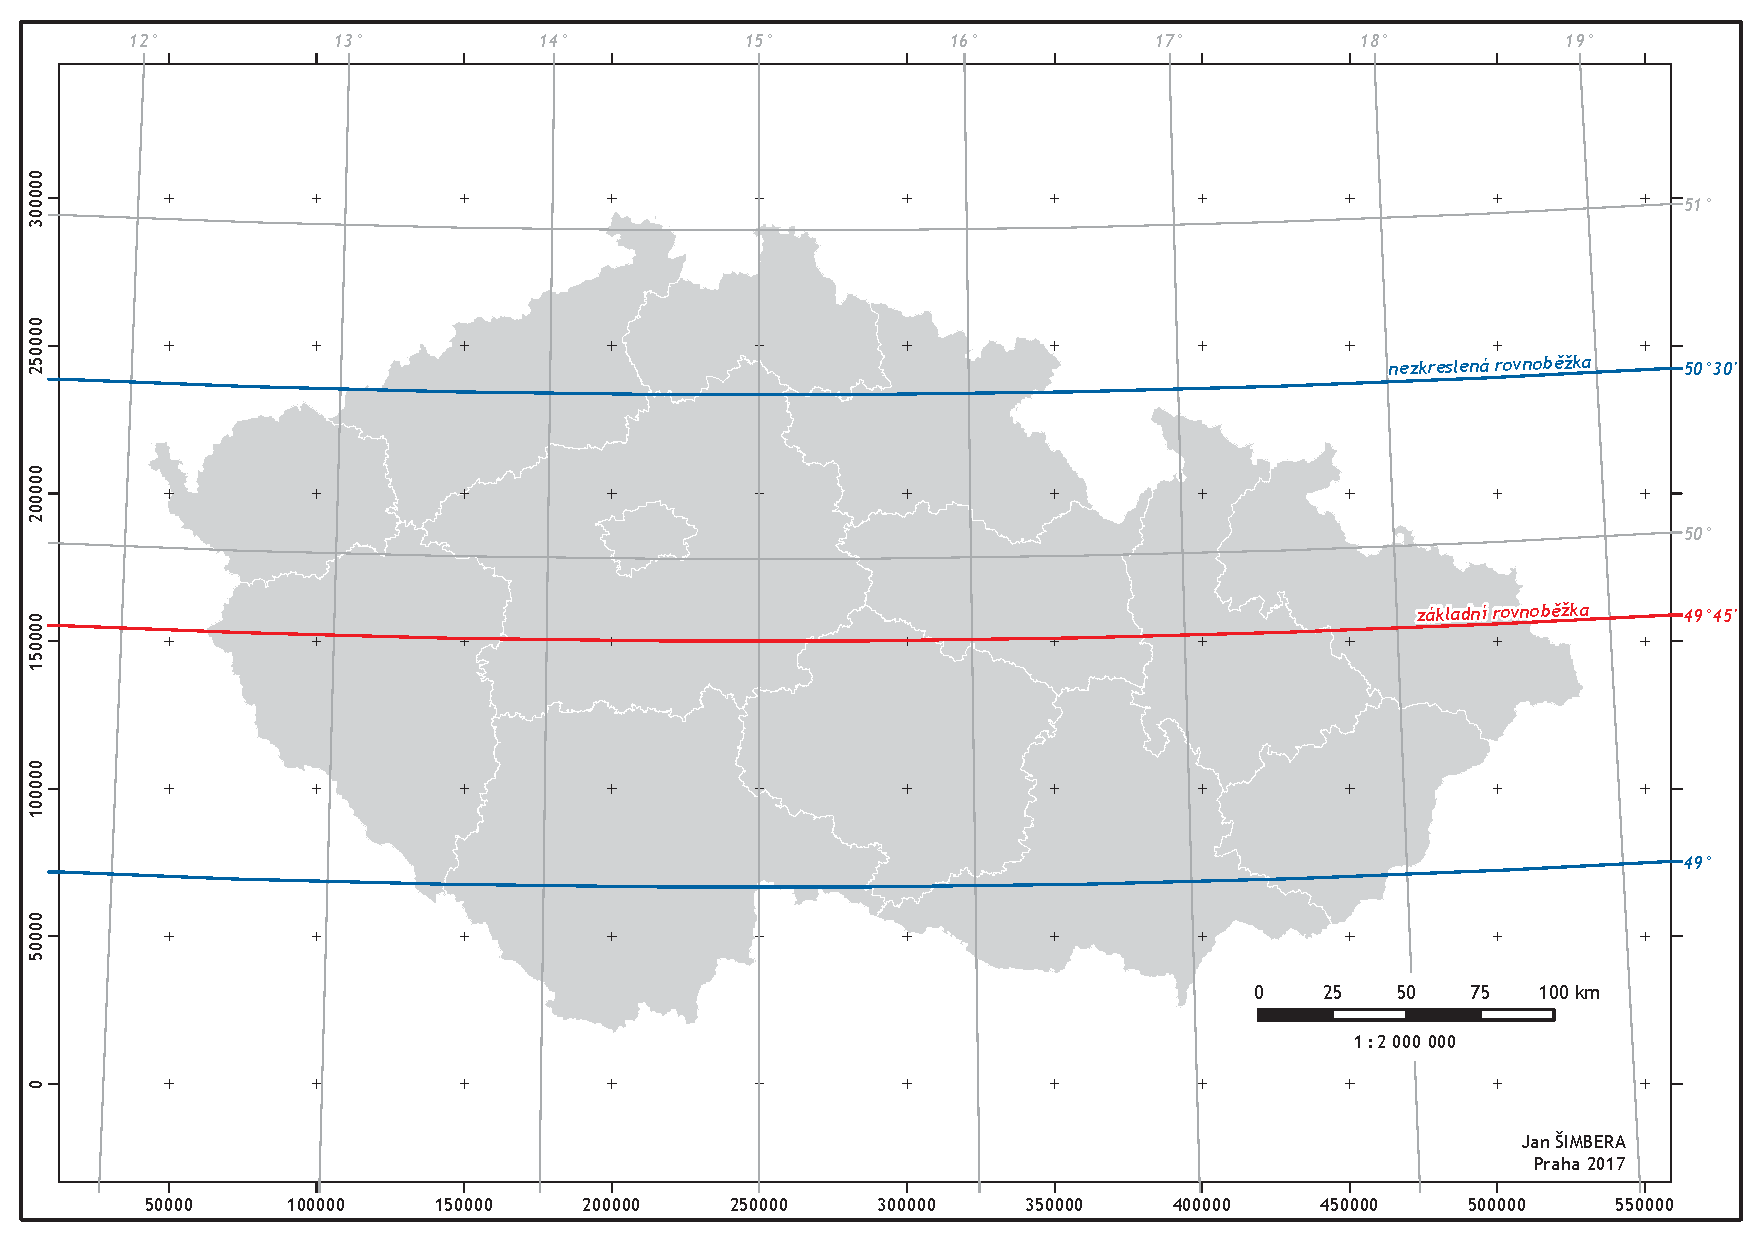
\includegraphics[width=1.25\textwidth]{map.pdf}}
\end{document}